\section{Il monitoraggio dell’energia software}

Il monitoraggio del consumo energetico a livello software rappresenta un tema di
ricerca centrale nell’ambito dell’efficienza energetica dei sistemi informatici moderni.
La crescente complessità delle architetture hardware e la diffusione di modelli di
calcolo dinamici e distribuiti hanno reso sempre più difficile ottenere misure
energetiche accurate e direttamente attribuibili alle singole componenti software.
Questo problema risulta particolarmente rilevante nel contesto del Serverless
Computing, dove le unità di esecuzione sono caratterizzate da invocazioni brevi,
stateless e altamente dinamiche.

Le soluzioni tradizionali di monitoraggio dell’energia si basano prevalentemente su
misurazioni a livello hardware, che forniscono una stima del consumo complessivo di
una macchina fisica o di specifici componenti, come CPU e memoria.
Sebbene tali approcci offrano un’elevata precisione, la loro granularità risulta spesso
insufficiente per analizzare il comportamento energetico delle applicazioni software,
soprattutto in ambienti multi-tenant e containerizzati \cite{lipp2021platypus}.
In questi scenari, il consumo energetico osservato è il risultato dell’interazione di
più entità software concorrenti, rendendo complessa l’attribuzione dei costi energetici
alle singole esecuzioni.

Per superare queste limitazioni, negli ultimi anni sono state proposte numerose
soluzioni di monitoraggio dell’energia software, che mirano a stimare il consumo
energetico a livelli di granularità più fini, quali processo, container o applicazione.
Tali approcci si basano generalmente su modelli di stima che correlano metriche
osservabili del sistema con misure energetiche ottenute a livello hardware, come nel
caso di PowerAPI e SmartWatts \cite{fieni:hal-02470128}.

Nel contesto del Serverless Computing, il problema del monitoraggio energetico è ulteriormente aggravato 
dalla crescente diffusione di architetture cloud-edge. 
Per ridurre la latenza e migliorare la qualità del servizio, 
sempre più spesso la computazione viene spostata verso nodi edge prossimi alla sorgente dei dati, 
anziché su data center remoti \cite{Shi2016_EdgeVisionChallenges}. 

Come già accennato, tali nodi sono frequentemente caratterizzati da risorse computazionali ed energetiche significativamente più limitate.
In questi scenari, la conoscenza del profilo energetico delle esecuzioni non è soltanto 
un'informazione utile ai fini dell'ottimizzazione, ma diventa un prerequisito per qualsiasi 
decisione consapevole sull'esecuzione. 
Le condizioni operative dei nodi edge possono variare nel tempo in funzione del 
carico di lavoro, delle caratteristiche dell'hardware sottostante e, in alcuni casi, 
della disponibilità energetica stessa del nodo. 
Di conseguenza, metriche energetiche statiche o ottenute tramite profilazione offline 
risultano spesso inadeguate a rappresentare il comportamento reale delle esecuzioni.
Diventa quindi fondamentale disporre di metriche energetiche aggiornate nel tempo, 
in grado di supportare decisioni di esecuzione che tengano conto sia del consumo energetico 
sia della qualità del risultato prodotto, ponendo le basi per politiche di scheduling 
capaci di gestire in modo controllato il compromesso tra queste due dimensioni.
\subsection{Misuratori hardware del consumo energetico}

I misuratori hardware del consumo energetico rappresentano l’approccio più diretto
per la misurazione dell’energia assorbita da un sistema di calcolo.
Tali soluzioni si basano su sensori fisici, esterni o integrati nell’hardware, e
forniscono misure caratterizzate da un’elevata accuratezza, in quanto l’energia viene
misurata direttamente a livello fisico.
Il monitoraggio può avvenire a livello di intera macchina o di specifici componenti
hardware, come CPU e memoria.

Una prima categoria è rappresentata dai misuratori hardware esterni, ovvero
dispositivi interposti fisicamente tra la sorgente di alimentazione e il sistema
sotto analisi.
Questi strumenti consentono di misurare l’energia realmente dissipata dall’intero
ecosistema hardware, includendo componenti spesso non osservabili tramite sensori
software, come gli alimentatori (PSU), i sistemi di raffreddamento e le perdite
resistive dei circuiti.
Per tale motivo, essi forniscono una visione completa del consumo energetico del
sistema.

Tuttavia, come ampiamente documentato in letteratura \cite{freina2024energysurvey}, l’adozione di misuratori
hardware esterni introduce una serie di criticità che ne limitano l’applicabilità in
contesti operativi su larga scala.
In primo luogo, la misurazione avviene tipicamente a livello di intero sistema
(\textit{full-system power}), rendendo complesso isolare il contributo energetico di
singoli componenti hardware o di specifiche entità software senza ricorrere a
strumentazione aggiuntiva e altamente invasiva.
In secondo luogo, l’integrazione di tali dispositivi in infrastrutture distribuite o
in ambienti di data center comporta costi economici e complessità operative
significative, legate sia all’acquisizione dell’hardware sia alla gestione del
cablaggio e della raccolta dei dati.

Per fornire un ordine di grandezza dell’investimento richiesto, nella Tabella
\ref{tab:costi_hardware} sono riportate alcune delle principali categorie di strumenti
utilizzati per il monitoraggio energetico hardware, insieme ai relativi ambiti di
applicazione.

\begin{table}[t]
\centering
\caption{Confronto tra principali tipologie di misuratori hardware esterni per il
monitoraggio del consumo energetico.}
\label{tab:costi_hardware}
\begin{tabular}{|l|p{4cm}|p{3cm}|p{4cm}|}
\hline
\textbf{Categoria} & \textbf{Esempio di Dispositivo} & \textbf{Costo Stimato} & \textbf{Ambito di utilizzo} \\ \hline
Entry-level &
TP-Link Kasa, Kill-A-Watt &
€30 -- €60 &
Analisi preliminari e misure indicative su singole workstation. \\ \hline
Enterprise &
APC Metered Rack PDU, Raritan PX &
€800 -- €2.500 &
Monitoraggio energetico di rack o gruppi di server in data center. \\ \hline
Laboratorio / R\&D &
Yokogawa WT310E, ZES ZIMMER LMG &
€2.500 -- €6.000+ &
Misurazioni ad alta precisione per validazione scientifica e ricerca accademica. \\ \hline
\end{tabular}
\end{table}

I dispositivi di fascia entry-level offrono generalmente frequenze di campionamento
limitate, dell’ordine di pochi Hertz, risultando adeguati per analisi preliminari su
singole macchine.
Al contrario, gli strumenti utilizzati in ambito di ricerca e validazione
scientifica consentono misurazioni ad alta frequenza e un’elevata precisione, a
fronte di costi significativamente più elevati.

Oltre ai misuratori hardware esterni, i moderni processori integrano sensori
energetici direttamente a livello di chip, rendendo possibile l’accesso a stime
del consumo energetico tramite interfacce software.
Un esempio significativo è rappresentato dalla tecnologia \textit{Running Average
Power Limit} (RAPL), introdotta da Intel, che consente di ottenere informazioni
sul consumo energetico di diversi domini di potenza interni al processore
\cite{intel-rapl, rapl_description}.

RAPL suddivide il consumo energetico del sistema in un insieme di domini logici,
ciascuno dei quali rappresenta una porzione specifica dell’hardware.
In particolare, il dominio \textit{Package} (PKG) rappresenta il consumo energetico
complessivo del processore, includendo i core, le cache e le interconnessioni interne.
Il dominio \textit{Power Plane 0} (PP0) è invece associato principalmente ai core
di calcolo della CPU, mentre altri domini, come \textit{DRAM}, forniscono una stima
del consumo energetico della memoria principale, quando supportati
dall’architettura.

La Figura~\ref{fig:rapl-domains} illustra un esempio di suddivisione del consumo
energetico secondo il modello RAPL, evidenziando come i diversi domini di potenza
corrispondano a specifiche componenti hardware del sistema.
Questa rappresentazione consente di comprendere come le misure fornite da RAPL
siano intrinsecamente legate all’organizzazione fisica del processore e non alle
singole entità software in esecuzione.

\begin{figure}[t]
    \centering
    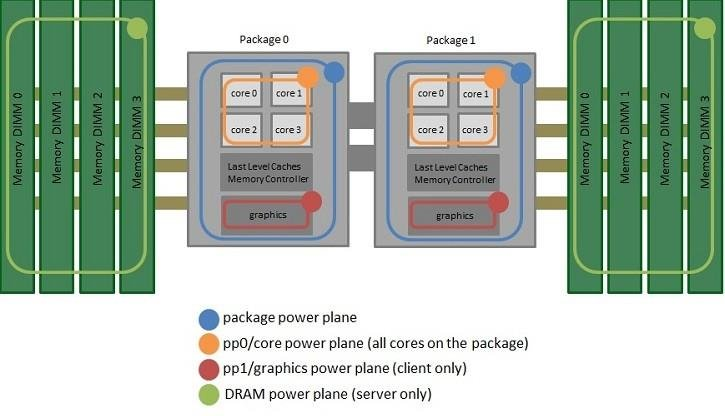
\includegraphics[width=0.8\textwidth]{figures/RAPL-Power-Domains-1.png.jpeg}
    \caption{Esempio di domini di potenza definiti dal modello RAPL. Il dominio
    \textit{Package} rappresenta il consumo energetico complessivo della CPU,
    mentre domini più specifici, come \textit{PP0} e \textit{DRAM}, forniscono
    stime riferite rispettivamente ai core di calcolo e alla memoria principale.}
    \label{fig:rapl-domains}
\end{figure}

Il funzionamento di RAPL si basa su modelli energetici interni al processore,
calibrati dal produttore, che stimano l’energia consumata a partire da eventi
hardware e contatori interni.
Sebbene tali misure non rappresentino una misurazione fisica diretta dell’energia,
diversi studi hanno dimostrato come esse offrano un buon compromesso tra accuratezza
e semplicità di utilizzo, risultando particolarmente adatte al monitoraggio
energetico a runtime\cite{rapl-evaluation}.
Le informazioni rese disponibili da RAPL possono essere lette tramite interfacce
standard del sistema operativo, consentendo la loro integrazione in strumenti di
monitoraggio software.

Nonostante questi vantaggi, i sensori hardware integrati presentano limiti
strutturali quando applicati a contesti software moderni.
La granularità delle misure è tipicamente limitata al livello di macchina o di
componente hardware e non consente di attribuire in modo diretto il consumo
energetico alle singole applicazioni, ai container o alle singole invocazioni.
In ambienti multi-tenant e containerizzati, come quelli tipici del Serverless
Computing, il consumo energetico osservato è quindi il risultato dell’esecuzione
concorrente di più entità software, rendendo complessa l’analisi del comportamento
energetico delle singole funzioni.

Inoltre, le misure fornite da RAPL sono di natura cumulativa e non distinguono in
modo esplicito tra le diverse fasi di esecuzione, quali inizializzazione,
esecuzione vera e propria e periodi di inattività.
Questo aspetto risulta particolarmente critico nel Serverless Computing, dove
fenomeni come il cold start e il riutilizzo dei container hanno un impatto
significativo sul consumo energetico complessivo.
Di conseguenza, pur costituendo una base affidabile per la stima dell’energia a
livello di sistema, i sensori hardware integrati non risultano sufficienti per
supportare analisi a grana fine e decisioni di gestione energetica a livello
software.


Alla luce di queste considerazioni, sebbene i misuratori hardware costituiscano una base affidabile per la misurazione dell’energia, essi risultano insufficienti per
supportare il monitoraggio continuo e a grana fine richiesto da ambienti dinamici e
distribuiti.
In tali contesti emerge la necessità di soluzioni in grado di offrire una maggiore
flessibilità e di integrarsi in modo più stretto con i meccanismi di esecuzione del
software.


\subsection{Misuratori software e modelli di stima}

Le limitazioni intrinseche dei misuratori hardware, quali la scarsa granularità
temporale, i costi elevati di implementazione su larga scala e l’impossibilità di
attribuire direttamente il consumo energetico a singole entità logiche in sistemi
multi-tenant, hanno favorito l’emergere dei misuratori software.
Questi strumenti non si basano su sensori fisici dedicati per ogni applicazione,
ma utilizzano modelli di stima che correlano l’attività del software con il consumo
energetico complessivo del sistema.
Il principio fondamentale consiste nell’impiegare metriche di utilizzo delle
risorse hardware — come cicli di clock della CPU, istruzioni eseguite, accessi alla
cache e operazioni di input/output — come base per stimare l’energia
assorbita dalle singole entità di esecuzione.
Questo approccio consente di ottenere una visibilità energetica più granulare
rispetto alle sole misure hardware, risultando particolarmente adatto a contesti
moderni quali il cloud computing, le architetture a microservizi e i sistemi
containerizzati.

Uno dei framework più rappresentativi in questo ambito è PowerAPI, una libreria modulare progettata per il monitoraggio del consumo energetico a livello di processo attraverso componenti indipendenti e meccanismi di raccolta dati asincroni e scalabili
\cite{fieni:hal-02470128}. L’architettura di PowerAPI è progettata per separare nettamente la fase di raccolta
delle metriche da quella di stima energetica, favorendo l’estendibilità e la
portabilità del sistema. Il pilastro tecnologico di PowerAPI è rappresentato dall’\textbf{HWPC Sensor}
(\textit{Hardware Performance Counter Sensor}), un componente specializzato nel
campionamento ad alta frequenza dei contatori di prestazione hardware
\cite{powerapi-hwpc}.
Il sensore si interfaccia direttamente con il sottosistema \texttt{perf\_event} del
kernel Linux, permettendo di raccogliere metriche dettagliate sull’attività della
CPU associate a specifici \textit{Control Groups} (cgroups)
\footnote{Il sottosistema \texttt{perf\_event} del kernel Linux fornisce
un’interfaccia unificata per il monitoraggio di eventi hardware e software a basso
livello, come cicli di clock della CPU, istruzioni eseguite e cache miss.
Attraverso la chiamata di sistema \texttt{perf\_event\_open()}, consente di associare
le misurazioni a processi, thread o \textit{cgroups}, esponendo i dati tramite
\textit{file descriptor} e buffer ad anello con overhead contenuto.
\texttt{perf\_event} costituisce inoltre la base del tool \texttt{perf}, ampiamente
utilizzato per la profilazione delle prestazioni nei sistemi Linux.} In parallelo, l’HWPC Sensor interroga i \textit{Model Specific Registers} (MSR)
tramite l’interfaccia \textit{Running Average Power Limit} (RAPL), ottenendo misure
cumulative del consumo energetico dei principali domini della CPU
\cite{rapl-evaluation}.

La Figura~\ref{fig:powerapi-architecture} mostra una rappresentazione concettuale
dell’architettura di PowerAPI.
Le metriche di utilizzo delle risorse e le informazioni energetiche fornite dai
sensori hardware vengono elaborate dal modello di stima \textbf{SmartWatts}, adottato
da PowerAPI per attribuire il consumo energetico ai singoli processi.

\begin{figure}[t]
    \centering
    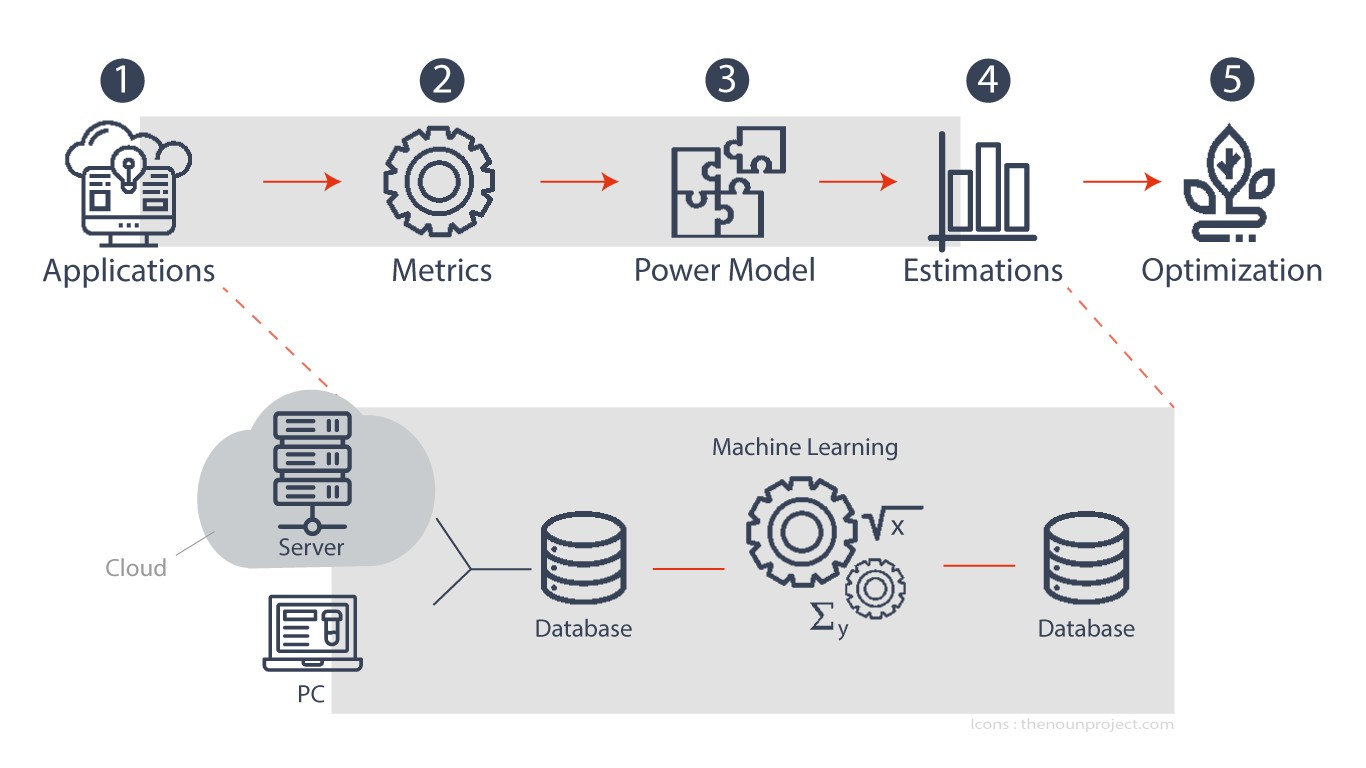
\includegraphics[width=0.9\textwidth]{figures/PowerApi.jpg}
    \caption{Architettura concettuale di PowerAPI. I contatori di prestazione hardware
    e le misure energetiche aggregate (RAPL) vengono combinati dal modello SmartWatts
    per stimare il consumo energetico dei singoli processi.}
    \label{fig:powerapi-architecture}
\end{figure}

SmartWatts utilizza tecniche di regressione lineare per scomporre il consumo
energetico globale in una componente statica e una dinamica, consentendo
un’attribuzione più accurata rispetto a modelli puramente statici
\cite{powerapi-smartwatts}.
Tale approccio richiede una fase di auto-calibrazione \textit{online} e l’accesso
diretto all’hardware sottostante.

Tali requisiti rendono PowerAPI particolarmente adatto a scenari \textit{bare-metal},
ma ne limitano l’applicabilità in ambienti virtualizzati e cloud pubblici, dove
l’accesso ai registri hardware della CPU e ai performance counter è spesso inibito
dagli hypervisor per motivi di sicurezza e isolamento.
In questi contesti emerge la necessità di strumenti di monitoraggio energetico
progettati nativamente per ambienti orchestrati.

Un approccio rappresentativo in questa direzione è \textbf{Kepler}
(\textit{Kubernetes-based Efficient Power Level Exporter}), un progetto
\textit{cloud-native} orientato al monitoraggio energetico di container e Pod in
cluster Kubernetes \cite{kepler-medium,kepler-redhat2}.
A differenza di PowerAPI, Kepler non richiede accesso diretto ai registri hardware
della CPU, ma sfrutta la tecnologia \textit{eBPF} (\textit{Extended Berkeley Packet
Filter}) per raccogliere metriche a livello kernel in modo non intrusivo e con
overhead computazionale ridotto.

La Figura~\ref{fig:kepler-architecture} mostra l’architettura complessiva di Kepler.
Il sistema utilizza un \textit{eBPF Program Generator} per generare dinamicamente
programmi eBPF che vengono agganciati ai \textit{tracepoint} del kernel e ai
performance counter della CPU.
Questi programmi intercettano eventi di schedulazione e statistiche di esecuzione,
consentendo di associare l’attività computazionale ai singoli container in modo
fine-grained.

Le informazioni raccolte tramite eBPF vengono arricchite dal \textit{Pod Lister},
che interroga le API di Kubernetes per mappare gli identificativi dei container ai
rispettivi Pod e raccoglie statistiche aggiuntive dai \textit{control groups}.
Parallelamente, il componente \textit{Energy Stats Reader} acquisisce informazioni
energetiche aggregate dal nodo, utilizzando diverse fonti a seconda della
disponibilità dell’hardware sottostante, tra cui RAPL, sensori hardware esterni,
interfacce GPU (NVML) e modelli basati su benchmark standardizzati.

Quando le misure hardware dirette non risultano accessibili, scenario tipico delle
macchine virtuali nei cloud pubblici, Kepler ricorre a modelli di stima basati su
\textit{Machine Learning}, denominati \textit{Estimators}.
Tali modelli, addestrati offline su differenti architetture hardware e carichi di
lavoro, ricevono in input le metriche raccolte a livello kernel e producono una
stima della potenza assorbita dai container, che viene successivamente integrata nel
tempo per ottenere una stima energetica complessiva.

Le metriche prodotte da Kepler vengono infine esposte tramite un \textit{Prometheus
Exporter}, rendendo il consumo energetico direttamente interrogabile attraverso i
meccanismi di \textit{scraping} standard e facilmente integrabile con strumenti di
visualizzazione.
Questa integrazione nativa con l’ecosistema di osservabilità cloud consente di
affiancare le metriche energetiche a quelle di performance, abilitando analisi
congiunte e politiche di gestione consapevoli dal punto di vista energetico.
\begin{figure}[t]
    \centering
    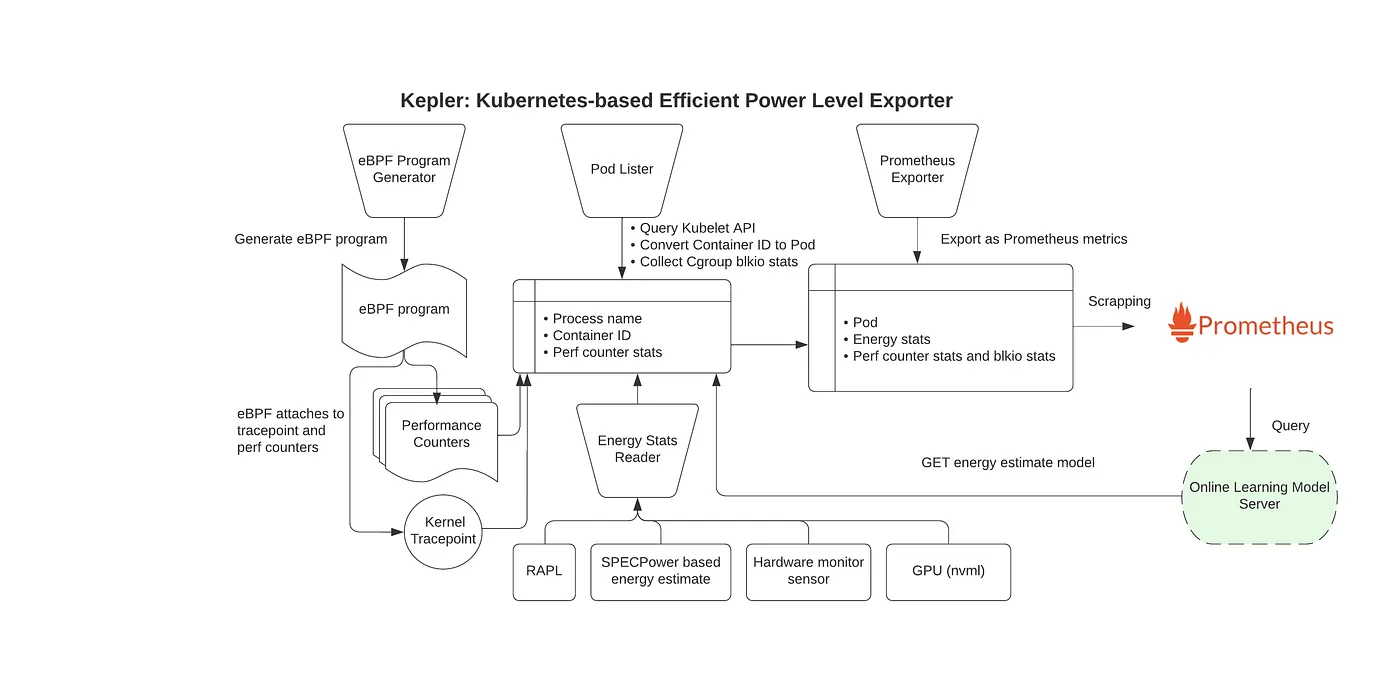
\includegraphics[width=0.75\textwidth]{figures/Kepler.png}
    \caption{Architettura di Kepler.}
    \label{fig:kepler-architecture}
\end{figure}

